\documentclass[14pt,a4paper]{extreport}

\usepackage[utf8]{inputenc}
\usepackage[romanian]{babel}

% \renewcommand\familydefault{\sfdefault} % computer modern sans serif
\usepackage{fontspec}
\setmainfont{Times New Roman}


\linespread{1}

\usepackage{geometry}
 \geometry{
 left=20mm,
 right=10mm,
 top=20mm,
 bottom=20mm,
 % showframe
}

\usepackage{xcolor}
\definecolor{mygreen}{rgb}{0,0.6,0}
\definecolor{mygray}{rgb}{0.5,0.5,0.5}
\definecolor{mymauve}{rgb}{0.58,0,0.82}
\definecolor{darkgray}{rgb}{.4,.4,.4}
\definecolor{navy}{HTML}{000080}
\definecolor{purple}{rgb}{0.65, 0.12, 0.82}
\definecolor{codepurple}{rgb}{0.58,0,0.82}
\definecolor{backcolour}{rgb}{0.95,0.95,0.92}

% Please add the following required packages to your document preamble:
\usepackage{multirow}
\usepackage{array}

\usepackage{caption}
% \usepackage[singlelinecheck=false]{caption}

% \captionsetup[table]{name=Tabelul}

\usepackage{graphicx}
\graphicspath{ {./} }

\usepackage{amsmath} % for the equation* environment

\usepackage{xcolor}   % for \textcolor
\usepackage{listings}
\lstset{
  columns=fullflexible,
  frame=single,
  breaklines=true,
  postbreak=\mbox{\textcolor{red}{$\hookrightarrow$}\space},
}

\begin{document}

\begin{titlepage}
\begin{center}
	{\large{ Universitatea Tehnica a Moldovei \\}}
	{\large{ Facultatea Calculatoare, Informatică și Microelectronică \\}}
	{\large{ Departamentul Ingineria Software și Automatică \\}}
	\vspace{4cm}
	{\LARGE {\bf{ Raport }}}\\
	\vspace{1cm}
	{\large { Lucrarea de Laborator Nr.6 \\}}
	{\normalsize { Varianta 1\\}}
	{\large { Programarea Orientată pe Obiecte\\}}
	{\large { Tema: Polimorfism. Funcţii virtuale \\}}
\end{center}

\vspace{5cm}

\noindent{\large A efectuat:\hfill St. gr. TI-206} \\
\noindent{\large\null\hfill Pleșu Cătălin} \\
\noindent{\null} \\
\noindent{\large A verificat:\hfill Lect. Univ.} \\
\noindent{\large\null\hfill Lisnic Inga} \\

\vspace{5cm}

\centering{\large{ Chișinău 2021 }}
\end{titlepage}

\clearpage

\paragraph{Listingul codului:}
\begin{verbatim*}
\lstinputlisting[language=C++]{main.cpp}
\end{verbatim*}
\lstinputlisting[language=C++]{main.cpp}

\paragraph{}
\begin{figure}[h]
\begin{center}
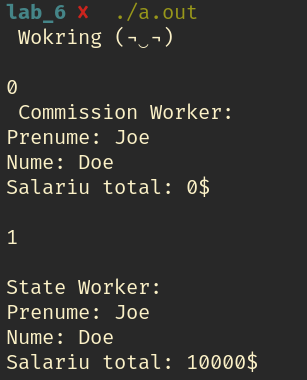
\includegraphics[width=11cm]{a1}
	\caption{Executarea programului pentru conditia a.} 
\end{center}
\end{figure}

\begin{figure}[h]
\begin{center}
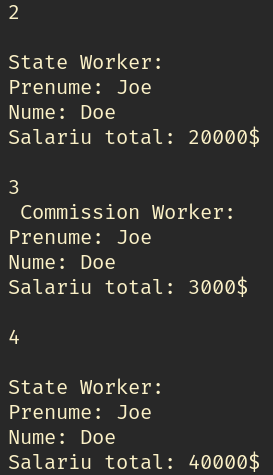
\includegraphics[width=11cm]{a2}
	\caption{Executarea programului pentru conditia a.} 
\end{center}
\end{figure}

\begin{figure}[h]
\begin{center}
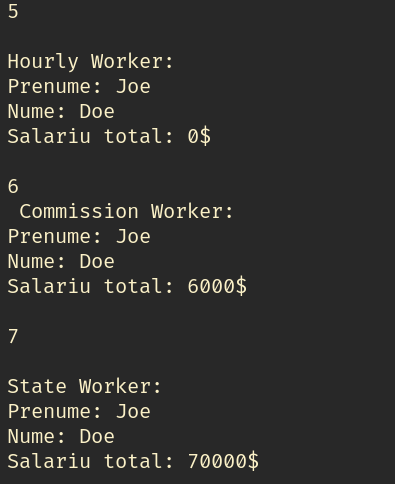
\includegraphics[width=11cm]{a3}
	\caption{Executarea programului pentru conditia a.} 
\end{center}
\end{figure}

\begin{figure}[h]
\begin{center}
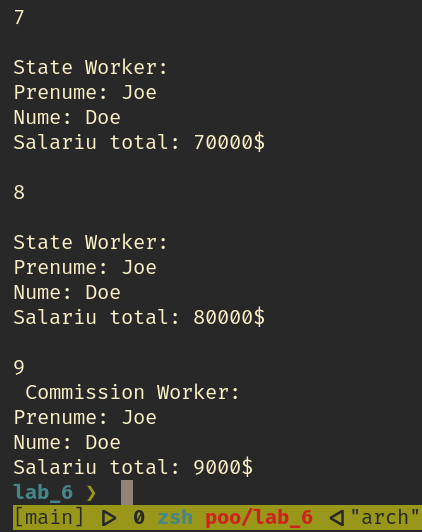
\includegraphics[width=11cm]{a4}
	\caption{Executarea programului pentru conditia a.} 
\end{center}
\end{figure}

\paragraph{}
\LaTeX

\end{document}
